\section{KHÔNG GIAN MẪU VÀ BIẾN CỐ}
\subsection{LÝ THUYẾT CẦN NHỚ}
\subsubsection{Phép thử ngẫu nhiên và không gian mẫu}
\begin{itemize}
	\item \textbf{Phép thử ngẫu nhiên} (gọi tắt là phép thử) là một thí nghiệm hay một hành động mà kết quả của nó không thể biết được trước khi phép thử được thực hiện.
	\item \textbf{Không gian mẫu} của phép thử (kí hiệu là $\Omega$) là tập hợp tất cả các kết quả có thể xảy ra khi thực hiện phép thử.
\end{itemize}
\indamm{Chú ý}: Ta chỉ xét phép thử mà không gian mẫu gồm hữu hạn kết quả.
\subsubsection{Biến cố}
\immini{
	\begin{itemize}
		\item \textbf{Biến cố} là một tập con của không gian mẫu $\Omega$, kí hiệu $A$, $B$, $C$,...
		\item Một kết quả thuộc tập $A$ được gọi là kết quả thuận lợi cho biến cố $A$. Số kết quả thuật lợi cho biến cố $A$ được kí hiệu là $n(A)$.
	\end{itemize}
	\indamm{Chú ý}
	\begin{itemize}
		\item \textbf{Biến cố chắc chắn} là biến cố luôn xảy ra, kí hiệu là $\Omega$.
		\item \textbf{Biến cố không thể} là biến cố không bao giờ xảy ra, ki hiệu là $\varnothing$.
	\end{itemize}
}{
	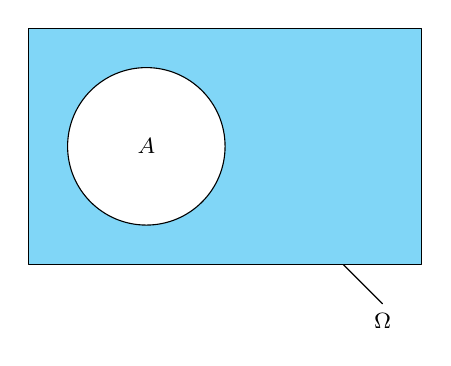
\begin{tikzpicture}[scale=1, font=\footnotesize, line join=round, line cap=round, >=stealth]
		\coordinate (A) at (0,0);
		\coordinate (B) at (5,0);
		\coordinate (C) at (5,3);
		\coordinate (D) at (0,3);
		\draw[fill=cyan!50] (A)--(B)--(C)--(D)--cycle;
		\draw(4,0)--(4.5,-.5) node[below] {$\Omega$};
		\filldraw[fill=white,draw=black] (1.5,1.5) circle (1cm);
		\fill (1.5,1.5) node{$A$};
\end{tikzpicture}}

\subsubsection{Biến cố đối}
Xét phép thử $T$  với không gian mẫu là  $\Omega$. Giả sử $E$ là một biến cố.
\begin{boxkn}
	\begin{itemize}
		\item  Biến cố đối của biến cố $E$ kí hiệu là $\overline{E}$. Nhận xét $\overline{E}=\Omega \backslash E$.
		\item Biến cố đối của biến cố $E$ là biến cố "$E$ không xảy ra". Nếu biến cố $E$ được mô tả dưới dạng mệnh đề toán học $Q$ thì biến cố đối $\overline{E}$ được mô tả bằng mệnh đề phủ định của mệnh đề $Q$ (tức là mệnh đề $\overline{Q}$).
	\end{itemize}
\end{boxkn}
\indamm{Nhận xét:} Nếu biến cố $E$ là tập con của không gian mẫu $\Omega$ thì $\overline{E}$ là phần bù của $E$ trong $\Omega$.
\begin{center}
	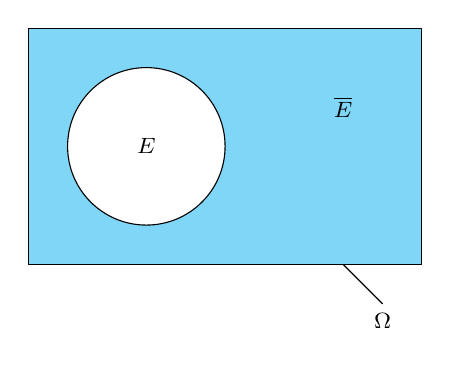
\begin{tikzpicture}[scale=1, font=\footnotesize, line join=round, line cap=round, >=stealth]
		\coordinate (A) at (0,0);
		\coordinate (B) at (5,0);
		\coordinate (C) at (5,3);
		\coordinate (D) at (0,3);
		\fill[cyan!10] (A)--(B)--(C)--(D);
		\draw[fill=cyan!50] (A)--(B)--(C)--(D)--cycle;
		\draw(4,0)--(4.5,-.5) node[below] {$\Omega$};
		\filldraw[fill=white,draw=black] (1.5,1.5) circle (1cm);
		\fill (1.5,1.5) node{$E$};
		\node at (4,2) {$\overline{E}$};
	\end{tikzpicture}
\end{center}


%-------------------------------------------------------------------------------------------------------------
\subsection{PHÂN LOẠI VÀ PHƯƠNG PHÁP GIẢI TOÁN}
\begin{dang}{Phép thử gieo đồng xu, gieo xúc xắc}
	\begin{listEX}[1]
		\item [\ding{172}] Đồng xu cân đối, đồng chất thường được quy ước bởi $2$ mặt \lq \lq sấp\rq \rq và \lq \lq ngửa\rq \rq.
		\item [\ding{173}] Con xúc xắc cân đối, đồng chất có $6$ mặt, mỗi mặt được kí hiệu với số chấm tương ứng.
	\end{listEX}
\end{dang}
%Ví dụ 1
\begin{vd}%[0D0H1-2]%[Dự án đề cương 3 khối NH24-25 - Đợt 4 - Quan Ón]
	Xét phép thử $T$ \lq\lq Gieo một con xúc xắc cân đối và đồng chất\rq\rq. 
	\begin{enumerate}
		\item Mô tả không gian mẫu.
		\item Gọi $A$ là biến cố \lq\lq Số chấm trên mặt xuất hiện là số chấm chẵn\rq\rq. Liệt kê tất cả các kết quả thuận lợi của biến cố $A$ và $\overline{A}$.
	\end{enumerate}
	\loigiai{
		\begin{enumerate}
			\item Không gian mẫu của phép thử là
			$\Omega = \{1;2;3;4;5;6\}$.
			\item Biến cố $A=\{2;4;6\}$.\\
			Suy ra biến cố đối của $A$ là $\overline{A}=\{1;3;5\}$.
		\end{enumerate}
	}
\end{vd}
%Ví dụ 2
\begin{vd}%[0D0H1-2]%[Dự án đề cương 3 khối NH24-25 - Đợt 4 - Quan Ón]
	Gieo một con xúc xắc cân đối, đồng chất liên tiếp hai lần.
	\begin{enumerate}
		\item Mô tả không gian mẫu.
		\item Gọi $A$ là biến cố \lq\lq Tổng số chấm xuất hiện lớn hơn hoặc bằng $8$\rq\rq. Liệt kê tất cả các kết quả thuận lợi của biến cố $A$.
	\end{enumerate}
	\loigiai{
	\begin{enumerate}
		\item Không gian mẫu của phép thử là
		$\Omega = \left\lbrace (i;j)\mid i;j=1,2,\ldots,6\right\rbrace$.
		\item Biến cố $A=\{(2;6),(3;5),(4;4),(5;3),(6;2),(3;6),(4;5),(6;3),(5;4),(4;6),(5;5),(6;4),(5;6),(6;5),(6;6)\}$.
	\end{enumerate}
	}
\end{vd}

%Ví dụ 3
\begin{vd}%[0D0H1-3]%[Dự án đề cương 3 khối NH24-25 - Đợt 4 - Quan Ón]
	Xét phép thử $T$ \lq\lq Gieo một đồng xu $3$ lần\rq\rq. 
	\begin{enumerate}
		\item Mô tả không gian mẫu. Tính số phần tử của tập không gian mẫu.
		\item Xác định phần tử của các biến cố và biến cố đối tương ứng của mỗi biến cố sau
		\begin{itemize}
			\item $A$: \lq\lq Ba lần gieo đều mặt sấp\rq\rq.
			\item $B$: \lq\lq Có đúng $2$ lần gieo xuất hiện mặt sấp\rq\rq.
		\end{itemize}
	\end{enumerate}
	\loigiai{
		\begin{enumerate}
			\item Không gian mẫu của phép thử là
			$$\Omega =\{NNN,NSN,SNN,SSN,NNS,NSS,SNS,SSS\}.$$
			Do đó số phần tử của không gian mẫu là $n\left(\Omega\right)=8$.
			\item Biến cố $A=\{SSS\}$.\\
			Suy ra biến cố đối của $A$ là $\overline{A}=\{NNN,NSN,SNN,SSN,NNS,NSS,SNS\}$.\\
			Biến cố $B=\{SSN,SNS,NSS\}$.\\
			Suy ra biến cố đối của $B$ là $\overline{B}=\{NNN,NSN,SNN,NNS,SSS\}$.
		\end{enumerate}
		}
\end{vd}

\begin{dang}{Một số phép thử đơn giản khác}
	Một số bài toán thường gặp
	\begin{listEX}[1]
		\item [\ding{172}] Bài toán về phép thử chọn số tự nhiên.
		\item [\ding{173}] Bài toán về phép thử chọn người, đồ vật,...
	\end{listEX}
\end{dang}

%Ví dụ 1
\begin{vd}%[0D0H1-2]%[Dự án đề cương 3 khối NH24-25 - Đợt 4 - Quan Ón]
	Chọn ngẫu nhiên một số nguyên dương không lớn hơn $25$.
	\begin{tasks}
		\task Mô tả không gian mẫu.
		\task Gọi $A$ là biến cố \lq\lq Số được chọn là số chính phương\rq\rq. Liệt kê tất cả các kết quả thuận lợi của biến cố $A$.
	\end{tasks}
	\loigiai{
	\begin{enumerate}
		\item Không gian mẫu là $\Omega =\{1;2;3;\ldots;25\}$.
		\item Biến cố $A=\{1;4;9;16;25\}$.
	\end{enumerate}
	}
\end{vd} 

%Ví dụ 2
\begin{vd}%[0D0H1-2]%[Dự án đề cương 3 khối NH24-25 - Đợt 4 - Quan Ón]
	Gọi $S$ là tập hợp các số tự nhiên có hai chữ số khác nhau được lập từ các chữ số $1$, $2$, $3$, $4$. Chọn ngẫu nhiên $1$ số từ tập $S$.
	\begin{enumerate}
		\item Mô tả không gian mẫu.
		\item Gọi $A$ là biến cố: \lq\lq Số lập được chia hết cho $3$\rq\rq. Liệt kê tất cả các kết quả thuận lợi của biến cố $A$.
	\end{enumerate}
	\loigiai{
		Các số tự nhiên có hai chữ số khác nhau được lập từ các chữ số $1$, $2$, $3$, $4$ là $S = \{12;13;14;21;23;24;31;32;34;41;42;43\}$.
	\begin{enumerate}
		\item Không gian mẫu là $\Omega = \{12;13;14;21;23;24;31;32;34;41;42;43\}$.
		\item Biến cố $A = \{12;21;24;42\}$.
	\end{enumerate}
	}
\end{vd}

%Ví dụ 3
\begin{vd}%[0D0H1-3]%[Dự án đề cương 3 khối NH24-25 - Đợt 4 - Quan Ón]
	Một hộp chứa bốn tấm thẻ được đánh số lần lượt là $1$, $2$, $3$, $4$ (mỗi thẻ chỉ đánh $1$ số). Lấy ngẫu nhiên hai thẻ từ hộp.
	\begin{enumerate}
		\item Xác định số phần tử của không gian mẫu. 
		\item Liệt kê tất cả các kết quả thuận lợi của các biến cố sau
		\begin{itemize}
			\item $H$: \lq\lq Tổng các số trên hai thẻ là số chẵn\rq\rq.
			\item $K$: \lq\lq Tích các số trên hai thẻ là số chẵn\rq\rq.
		\end{itemize}
	\end{enumerate}
	\loigiai{
	\begin{enumerate}
		\item Mỗi phần tử của không gian mẫu là một tổ hợp chập $2$ của $4$ phần tử trong tập hợp $\{1;2;3;4\}$.\\
		Do đó, số phần tử của không gian mẫu là $n(\Omega)= \mathrm{C}_4^{2}$.
		\item $H=\{(1;3),(2;4)\}$.\\
		$K=\{(1;2),(1;4),(2;3),(2;4),(3;4)\}$.
	\end{enumerate}
	}
\end{vd}
%-----------------------------------------------------------------------------
\subsection{Bài tập rèn luyện}
\ind{PHẦN I.} \inden{Câu trắc nghiệm nhiều phương án lựa chọn. Mỗi câu hỏi học sinh chỉ chọn một phương án.}\\
\setcounter{ex}{0}
\Opensolutionfile{ans}[ans/0T10-Bai1-TN]
\begin{ex}%[0D0N1-2]%[Dự án đề cương 3 khối NH25-26-Đợt 1-Lê Hồ Quang Minh]
	\textbf{(Trích đề thi HK2 - THPT Kiến Thụy – Hải Phòng – 2023–2024)}\\
	Gieo một đồng tiền có hai mặt S, N hai lần. Xác định biến cố $A$: \lq\lq Trong hai lần gieo có ít nhất một lần xuất hiện mặt $\mathrm{N}$\rq\rq.
	\choice
	{$A = \{NS; SN\}$}
	{$A = \{NS; NN\}$}
	{$A = \{NN\}$}
	{\True $A = \{NS; SN; NN\}$}
	\loigiai{
		Biến cố $A$: \lq\lq Trong hai lần gieo có ít nhất một lần xuất hiện mặt N\rq\rq $\Rightarrow A = \{NS; SN; NN\}$.
	}
\end{ex}

\begin{ex}%[0D0N1-3]%[Dự án đề cương 3 khối NH25-26-Đợt 1-Lê Hồ Quang Minh]
	\textbf{(Trích đề thi HK2 - THPT Trần Hưng Đạo – Hải Phòng – 2023-2024)}\\
	Gieo một xúc xắc cân đối và đồng chất một lần. Số phần tử của không gian mẫu $\Omega$ là
	\choice
	{$n(\Omega)=4$}
	{$n(\Omega)=8$}
	{\True $n(\Omega)=6$}
	{$n(\Omega)=10$}
	\loigiai{
		Số phần tử của không gian mẫu là $n(\Omega)=6$.
	}
\end{ex}

\begin{ex} %[0D0H1-3]%[Dự án đề cương 3 khối NH25-26-Đợt 1-Lê Hồ Quang Minh]
	\textbf{(Trích đề thi HK2 - THPT Nguyễn Huệ – Bà Rịa Vũng Tàu – 2023–2024)}\\
	Một hộp chứa $21$ viên bi kích thước như nhau, trong đó có $6$ viên bi màu xanh được đánh số từ $1$ đến $6$; có $7$ viên bi màu đỏ được đánh số từ $4$ đến $10$ và $8$ viên bi màu vàng được đánh số từ $9$ đến $16$. Lấy ngẫu nhiên $2$ viên bi từ hộp. Số phần tử của biến cố \lq\lq lấy $2$ viên bi vừa khác màu, vừa khác số\rq\rq\, là
	\choice
	{$135$}
	{\True $141$}
	{$137$}
	{$138$}
	\loigiai{
		Số cách lấy $2$ viên bi bất kì là $\mathrm{C}_{21}^{2} = 210$.\\
		Số cách lấy $2$ viên bi cùng màu là $\mathrm{C}_6^2 + \mathrm{C}_7^2 + \mathrm{C}_8^2 = 64$.\\
		Số cách lấy $2$ viên bi khác màu mà cùng số là $5$.\\
		Vậy số cách lấy $2$ viên bi khác màu và khác số là $210 - 64 - 5 = 141$.
	}
\end{ex}

\begin{ex}%[0D0N1-2]%[Dự án đề cương 3 khối NH25-26-Đợt 1-Lê Hồ Quang Minh]
	\textbf{(Trích đề thi HK2 - THPT Việt Nam – Ba Lan – 2023–2024)}\\
	Gieo một con xúc xắc cân đối, đồng chất. Gọi $A$ là biến cố \lq \lq xúc xắc xuất hiện mặt có số chấm không nhỏ hơn $3$\rq \rq. Khẳng định nào sau đây đúng?
	\choice
	{$A = \{1;2;3\}$}
	{$A = \{2;3\}$}
	{\True $A = \{3;4;5;6\}$}
	{$A = \{3;4;5\}$}
	\loigiai{
		Các mặt của con xúc xắc là $\{1;2;3;4;5;6\}$ nên không nhỏ hơn $3$ là $\{3;4;5;6\}$.
	}
\end{ex}

\begin{ex}%[0D0H1-3]%[Dự án đề cương 3 khối NH25-26-Đợt 1-Lê Hồ Quang Minh]
	\textbf{(Trích đề thi HK2 - THPT Nam Trực – Nam Định – 2023–2024)}\\
	Có $2024$ tấm thẻ được đánh số từ $1$ đến $2024$. Xét phép thử lấy ngẫu nhiên đồng thời $5$ tấm thẻ trong số $2024$ tấm thẻ đã cho. Số phần tử của không gian mẫu là
	\choice
	{$n(\Omega) = \mathrm{A}_{2024}^5$}
	{$n(\Omega) = \mathrm{C}_{2024}^1$}
	{$n(\Omega) = \mathrm{A}_{2024}^1$}
	{\True $n(\Omega) = \mathrm{C}_{2024}^5$}
	\loigiai{
		Số phần tử của không gian mẫu là $n(\Omega) = \mathrm{C}_{2024}^5$.
	}
\end{ex}

\begin{ex}%[0D0N1-2]%[Dự án đề cương 3 khối NH25-26-Đợt 1-Lê Hồ Quang Minh]
	\textbf{(Trích đề thi HK2 - THPT Tân Châu – An Giang – 2023–2024)}\\
	Xét phép thử tung một đồng xu ba lần. Xác định không gian mẫu của phép thử.
	\choice
	{$\Omega = \{\mathrm{S};\mathrm{N};\mathrm{SS};\mathrm{NN};\mathrm{SSN};\mathrm{NSN};\mathrm{NNS};\mathrm{SNN};\mathrm{SNS};\mathrm{NSS};\mathrm{NNN};\mathrm{SSS}\}$}
	{\True $\Omega = \{\mathrm{SNN};\mathrm{NSN};\mathrm{NNS};\mathrm{SSN};\mathrm{SNS};\mathrm{NSS};\mathrm{NNN};\mathrm{SSS}\}$}
	{$\Omega = \{\mathrm{S};\mathrm{NS};\mathrm{NNS}\}$}
	{$\Omega = \{\mathrm{N};\mathrm{NN};\mathrm{NNN};\mathrm{S};\mathrm{SS};\mathrm{SSS}\}$}
	\loigiai{
		Khi gieo một đồng xu chỉ có $2$ khả năng xảy ra, đó là sấp (S) hoặc ngửa (N).\\
		Vậy không gian mẫu là $\Omega = \{\mathrm{SNN};\mathrm{NSN};\mathrm{NNS};\mathrm{SSN};\mathrm{SNS};\mathrm{NSS};\mathrm{NNN};\mathrm{SSS}\}$.
	}
\end{ex}

\begin{ex}%[0D0N1-2]%[Dự án đề cương 3 khối NH25-26-Đợt 1-Lê Hồ Quang Minh]
	Gieo ngẫu nhiên một đồng xu cân đối và đồng chất hai lần. Kí hiệu mặt ngửa là $N$ và mặt sấp là $S$. Không gian mẫu của phép thử là
	\choice
	{$\Omega=\left\{S,N\right\}$}
	{\True $\Omega=\left\{SS,NN,SN,NS\right\}$}
	{$\Omega=\left\{SN,NS\right\}$}
	{$\Omega=\left\{SS,NN\right\}$}
	\loigiai{
		Gieo ngẫu nhiên hai lần có $4$ kết quả có thể xảy ra, nên tập hợp các phần tử của không gian mẫu là $\Omega=\left\{SS,NN,SN,NS\right\}$.
	}
\end{ex}


\begin{ex}%[0D0N1-2]%[Dự án đề cương 3 khối NH25-26-Đợt 1-Lê Hồ Quang Minh]
	Gieo đồng thời một đồng xu cân đối đồng chất và một con xúc xắc cân đối đồng chất. Không gian mẫu của phép thử trên là
	\choice
	{$\{1;2;3;4;5;6\}$}
	{$\{NN,NS,SN,SS\}$}
	{$\{S;N\}$}
	{\True $\{1S,2S,3S,4S,5S,6S,1N,2N,3N,4N,5N,6N\}$}
	\loigiai{
		Không gian mẫu của phép thử đã cho là $$\Omega=\{1S,2S,3S,4S,5S,6S,1N,2N,3N,4N,5N,6N\}.$$
	}
\end{ex}

\begin{ex}%[0D0H1-3]%[Dự án đề cương 3 khối NH25-26-Đợt 1-Lê Hồ Quang Minh]
	Gieo ngẫu nhiên một đồng xu cân đối và đồng chất $5$ lần. Tính số phần tử không gian mẫu.
	\choice
	{$ 64 $}
	{$ 16 $}
	{$ 10 $}
	{\True $ 32 $}
	\loigiai
	{
		Theo quy tắc nhân có $2^5=32$ cách.
	}
\end{ex}

\begin{ex}%[0D0N1-2]%[Dự án đề cương 3 khối NH25-26-Đợt 1-Lê Hồ Quang Minh]
	Gieo một con xúc xắc cân đối, đồng chất. Biến cố nào sau đây là biến cố chắc chắn
	\choice
	{$A$: \lq \lq Xuất hiện mặt chẵn chấm\rq \rq}
	{\True $C$: \lq \lq Xuất hiện mặt nhỏ hơn $7$ chấm\rq \rq}
	{$D$: \lq \lq Xuất hiện mặt có số chấm là một số nguyên tố\rq \rq}
	{$B$: \lq \lq Xuất hiện mặt lẻ chấm\rq \rq}
	\loigiai
	{
		Biến cố chắc chắn là $C$: \lq\lq Xuất hiện mặt nhỏ hơn $7$ chấm\rq\rq.
	}
\end{ex}

\begin{ex}%[0D0N1-3]%[Dự án đề cương 3 khối NH25-26-Đợt 1-Lê Hồ Quang Minh]
	Gieo một con xúc xắc $2$ lần. Số phần tử của không gian mẫu là
	\choice
	{\True $36$}
	{$12$}
	{$6$}
	{$18$}
	\loigiai{
		Số phần tử của không gian mẫu là$n(\Omega) = 6\cdot 6 = 36$.
	}
\end{ex}

\begin{ex}%[0D0H1-2]%[Dự án đề cương 3 khối NH25-26-Đợt 1-Lê Hồ Quang Minh]
	Gieo con xúc xắc hai lần. Biến cố $A$ là biến cố để sau hai lần gieo có ít nhất một mặt $6$ chấm xuất hiện. Biến cố $A$ là tập nào sau đây?
	\choice
	{$A=\{(1;6),(2;6),(3;6),(4;6),(5;6),(6;6)\}$}
	{\True $A=\{(1;6),(2;6),(3;6),(4;6),(5;6),(6;6),(6;1),(6;2),(6;3),(6;4),(6;5)\}$}
	{$A=\{(1;6),(2;6),(3;6),(4;6),(5;6),(6;1),(6;2),(6;3),(6;4),(6;5)\}$}
	{$A=\{(1;6),(2;6),(3;6),(4;6),(5;6)\}$}
	\loigiai
	{ Gieo con xúc xắc hai lần. Biến cố $A$ là biến cố để sau hai lần gieo có ít nhất một mặt $6$ chấm xuất hiện là  $A=\{(1;6),(2;6),(3;6),(4;6),(5;6),(6;6),(6;1),(6;2),(6;3),(6;4),(6;5)\}$.
	}
\end{ex}

\begin{ex}%[0D0H1-3]%[Dự án đề cương 3 khối NH25-26-Đợt 1-Lê Hồ Quang Minh]
	Gieo một con xúc xắc liên tiếp hai lần. Gọi $A$ là biến cố \lq \lq Kết quả hai lần gieo như nhau\rq \rq. Tính số phần tử của biến cố $A$.
	\choice
	{$n(A)=8$}
	{$n(A)=12$}
	{\True $n(A)=6$}
	{$n(A)=1$}
	\loigiai{
		Ta có $A=\left\{(1;1),(2;2),(3;3),(4;4),(5;5),(6;6)\right\}\Rightarrow n(A)=6$.
	}
\end{ex}

\begin{ex}%[0D0N1-3]%[Dự án đề cương 3 khối NH25-26-Đợt 1-Lê Hồ Quang Minh]
	Xét phép thử tung con xúc xắc $6$ mặt hai lần. Số phần tử của biến cố $B$: \lq\lq Tổng số chấm xuất hiện ở hai lần tung chia hết cho $3$\rq\rq\, là
	\choice
	{$n(B)=14$}
	{$n(B)=15$}
	{$n(B)=13$}
	{\True $n(B)=12$}
	\loigiai{
		Xét các cặp $(i,j)$ với $i,j\in \left\{1,2,3,4,5,6\right\}$ mà $(i+j)\vdots 3$.\\
		Ta có các cặp có tổng chia hết cho $3$ là $(1,2);(1,5);(2,4);(3,3);(3,6);(4,5);(6;6)$.\\
		Hơn nữa mỗi cặp (trừ cặp $(3,3)$; $(6;6)$) khi hoán vị ta được một cặp thỏa yêu cầu bài toán.\\
		Vậy $n(B)=12$.
	}
\end{ex}

\begin{ex}%[0D0H1-3]%[Dự án đề cương 3 khối NH25-26-Đợt 1-Lê Hồ Quang Minh]
	Minh muốn gọi điện cho Ngọc nhưng Minh quên mất chữ số cuối cùng của số điện thoại. Minh chọn ngẫu nhiên một chữ số cho chữ số cuối cùng để gọi thử. Tính số phần tử của không gian mẫu.
	\choice
	{$n(\Omega)=9$}
	{\True $n(\Omega)=10$}
	{$n(\Omega)=1$}
	{$n(\Omega)=11$}
	\loigiai{
		Không gian mẫu của phép thử $\Omega = \{0;1;2;3;4;5;6;7;8;9\}$ nên $n(\Omega)=10$.
		
	}
\end{ex}

\begin{ex}%[0D0H1-3]%[Dự án đề cương 3 khối NH25-26-Đợt 1-Lê Hồ Quang Minh]
	Danh sách lớp của bạn Nam được đánh số từ $1$ đến $45$. Nam có số thứ tự là $21$. Chọn ngẫu nhiên một bạn trong lớp để trực nhật. Gọi biến cố $B$: \lq\lq Bạn được chọn có số thứ tự lớn hơn số thứ tự của Nam\rq\rq. Chọn mệnh đề \textbf{sai}.
	\choice
	{Có $20$ bạn có số thứ tự nhỏ hơn số thứ tự của Nam}
	{\True Có $23$ bạn có số thứ tự lớn hơn số thứ tự của Nam}
	{Có $24$ kết quả thuận lợi cho biến cố $B$}
	{Tập hợp các kết quả chỉ số thứ tự của bạn được chọn lớn hơn số thứ tự của Nam là $\{22; 23; \ldots; 45\}$}
	\loigiai{
		Tập hợp các kết quả chỉ số thứ tự của bạn được chọn lớn hơn số thứ tự của Nam là $\{22; 23; \ldots; 45\}$.\\
		Tập hợp này có $45 - 22 + 1 = 24$ (phần tử) nên có $24$ bạn có số thứ tự lớn hơn số thứ tự của Nam.
	}
\end{ex}


\begin{ex}%[0D0H1-3]%[Dự án đề cương 3 khối NH25-26-Đợt 1-Lê Hồ Quang Minh]
	Có hai hộp chứa các quả bóng. Hộp thứ nhất chứa $4$ quả bóng được đánh số từ $1$ đến $4$. Hộp thứ hai chứa $5$ quả bóng được đánh số từ $1$ đến $5$. Chọn ngẫu nhiên từ mỗi hộp $1$ quả bóng. Có bao nhiêu kết quả thuận lợi cho biến cố \lq\lq Tổng các số ghi trên hai quả bóng không vượt quá $7$\rq\rq?
	\choice
	{\True $17$}
	{$15$}
	{$13$}
	{$16$}
	\loigiai{
		Tổng số các kết quả có thể xảy ra khi chọn bóng là $4 \cdot 5=20$.\\
		Có $3$ kết quả thuận lợi cho biến cố \lq\lq Tổng các số ghi trên hai quả bóng lớn hơn $7$\rq\rq\, nên số các kết quả thuận lợi cho biến cố \lq\lq Tổng các số ghi trên hai quả bóng không vượt quá $7$\rq\rq\, là $20-3=17$.
	}
\end{ex}

\begin{ex}%[0D0H1-3]%[Dự án đề cương 3 khối NH25-26-Đợt 1-Lê Hồ Quang Minh]
	Có hai hộp chứa các viên bi, hộp thứ nhất chứa $6$ viên bi và hộp thứ hai chứa $8$ viên bi. Xét phép thử ngẫu nhiên lấy mỗi hộp $2$ viên bi. Số phần tử của không gian mẫu là
	\choice
	{$n(\Omega) = \mathrm{C}_{14}^4$}
	{$n(\Omega) = \mathrm{C}_6^4 + \mathrm{C}_8^4$}
	{$n(\Omega) = \mathrm{C}_6^2 + \mathrm{C}_8^2$}
	{\True $n(\Omega) = \mathrm{C}_6^2 \cdot \mathrm{C}_8^2$}
	\loigiai{
		Lấy $2$ viên bi từ hộp thứ nhất có $\mathrm{C}_6^2$ (cách).\\
		Lấy $2$ viên bi từ hộp thứ hai có $\mathrm{C}_8^2$ (cách).\\
		Theo quy tắc nhân ta có $n(\Omega) = \mathrm{C}_6^2 \cdot \mathrm{C}_8^2$.
	}
\end{ex}

\begin{ex}%[0D0V1-3]%[Dự án đề cương 3 khối NH25-26-Đợt 1-Lê Hồ Quang Minh]
	Xét phép thử lấy ngẫu nhiên một số từ tập hợp tất cả các số tự nhiên có $5$ chữ số mà các chữ số đều khác $0$. 
	Gọi $A$ là biến cố \lq \lq Số lấy được chỉ có mặt ba chữ số khác nhau\rq \rq\,. Số phần tử của $A$ là
	\choice
	{$5\,040$}
	{$1\,400$}
	{\True $12\,600$}
	{$7\,560$}
	\loigiai{
		\textbf{Trường hợp 1:} Một trong $3$ chữ số có mặt đúng $3$ lần\\
		Chọn $1$ số trong $9$ chữ số và chọn $3$ vị trí để xếp số này có $9 \cdot \mathrm{C}_5^3$ cách.\\
		Chọn $2$ số khác nhau trong $8$ số còn lại để xếp vào $2$ vị trí còn lại có $\mathrm{A}_8^2$.\\
		Suy ra có $9 \cdot \mathrm{C}_5^3 \cdot \mathrm{A}_8^2 = 5\,040$ (số).\\
		\textbf{Trường hợp 2:} Hai trong $3$ chữ số mà mỗi chữ số có mặt hai lần, chữ số còn lại có mặt đúng một lần.\\
		Chọn $2$ số trong $9$ số và chọn vị trí để xếp $2$ số này, mỗi số $2$ vị trí có $\mathrm{C}_9^2 \cdot \mathrm{C}_5^2 \cdot \mathrm{C}_3^2$.\\
		Chọn $1$ số trong $7$ số còn lại và xếp vào $1$ vị trí còn lại có $7$ cách.\\
		Vậy có $\mathrm{C}_9^2 \cdot \mathrm{C}_5^2 \cdot \mathrm{C}_3^2 \cdot 7 = 7\,560$ cách.\\
		Số phần tử của $A$ là $5\,040 + 7\,560 = 12\,600$.
	}
\end{ex}

\begin{ex}%[0D0V1-3]%[Dự án đề cương 3 khối NH25-26-Đợt 1-Lê Hồ Quang Minh]
	Chọn ngẫu nhiên một số tự nhiên chẵn có bốn chữ số khác nhau từ tập $A = \{0;1;2;3;4;5;6\}$. Hỏi không gian mẫu có bao nhiêu phần tử?
	\choice
	{\True $420$}
	{$360$}
	{$120$}
	{$480$}
	\loigiai{
		Gọi số tự nhiên có $4$ chữ số là $x=\overline{abcd}$, $a \ne b \ne c \ne d$ và $a \ne 0$.\\
		Do $x$ là số chẵn nên $d \in \{0; 2; 4; 6\}$
		\begin{itemize}
			\item \textbf{Trường hợp 1:} $d = 0$ nên có $1$ cách chọn $d$.\\
			Còn lại $3$ vị trí $a,b,c$ ta chọn $3$ chữ số từ tập $A \setminus \{0\}$. Có $\mathrm{A}_6^3 = 120$ cách.\\
			Theo quy tắc nhân ta có $1 \cdot 120 = 120$ số.
			\item \textbf{Trường hợp 2:} $d \in \{2;4;6\}$: có $3$ cách chọn $d$.\\
			Vì $a \ne 0$ nên $a$ có $5$ cách chọn.\\
			Khi đó $b$, $c$ có $\mathrm{A}_5^2 = 20$ cách.\\
			Theo quy tắc nhân ta có $3 \cdot 5 \cdot 20 = 300$ số.
		\end{itemize}
		Suy ra có $120 + 300 = 420$ số tự nhiên cần tìm.\\
		Vậy số phần tử của không gian mẫu là $420$.
	}
\end{ex}
\Closesolutionfile{ans}
%\indapan{10}{ans/0T10-Bai1-TN}

\ind{PHẦN II.} \inden{Câu trắc nghiệm đúng sai. Trong mỗi ý a), b), c), d) ở mỗi câu, học sinh chọn đúng hoặc sai.}\\
\setcounter{ex}{0}
\Opensolutionfile{ans}[ans/0T10-Bai1-DS]

\begin{ex}%[0D0H1-3]%[Dự án đề cương 3 khối NH25-26-Đợt 1-Lê Hồ Quang Minh]
	\textbf{(Trích đề thi HK2 - THPT Lê Quý Đôn – Bà Rịa Vũng Tàu – 2023–2024)}\\
	Gieo một con xúc xắc $6$ mặt cân đối và đồng chất một lần.
	\choiceTF
	{\True Gọi $A$ là biến cố \lq\lq Số chấm xuất hiện trên con xúc xắc là $8$\rq\rq, khi đó $n(A) = 0$}
	{Số phần tử của không gian mẫu $n(\Omega) = 12$}
	{Gọi $C$ là biến cố \lq\lq Số chấm xuất hiện trên con xúc xắc lớn hơn $4$\rq\rq, khi đó $n(C) = 1$}
	{\True Gọi $B$ là biến cố \lq\lq Số chấm xuất hiện trên con xúc xắc là một số lẻ\rq\rq, khi đó $n(B) = 3$}
	\loigiai{
		\begin{itemchoice}
			\itemch \textbf{Đúng}. Vì $A = \varnothing$ do xúc xắc không có mặt số $8$, nên $n(A) = 0$.
			\itemch \textbf{Sai}. Vì xúc xắc 6 mặt nên $n(\Omega) = 6$.
			\itemch \textbf{Sai}. Vì xúc xắc có các mặt có số chấm lớn hơn $4$ là $5$, $6$, nên $n(C) = 2$.
			\itemch \textbf{Đúng}. Vì xúc xắc có các mặt có số chấm là số lẻ là $1$, $3$, $5$, nên $n(B) = 3$.
		\end{itemchoice}
	}
\end{ex}

\begin{ex}%[0D0H1-3]%[Dự án đề cương 3 khối NH25-26-Đợt 1-Lê Hồ Quang Minh]
	\textbf{(Trích đề thi HK2 – THPT Trần Hưng Đạo – Hải Phòng – 2023–2024)}\\
	Gieo một con xúc xắc $6$ mặt cân đối và đồng chất hai lần liên tiếp.
	\choiceTF
	{\True $n(\Omega) = 36$}
	{\True Gọi $A$ là biến cố \lq \lq Số chấm trong hai lần gieo đều là số lẻ\rq \rq, khi đó $n(A) = 9$}
	{ Gọi $B$ là biến cố \lq \lq Số chấm xuất hiện ở cả hai lần gieo giống nhau\rq \rq, khi đó $n(B) = 9$}
	{\True Gọi $C$ là biến cố \lq \lq Có ít nhất một lần gieo xuất hiện mặt một chấm\rq \rq, khi đó $n(C) = 11$}
	\loigiai{
		\begin{itemchoice}
			\itemch \textbf{Đúng}. Vì $n(\Omega) = 6\cdot 6 = 36$.
			\itemch \textbf{Đúng}. Vì số lẻ là $1,3,5$, nên $n(A) = \mathrm{C}_3^1 \cdot \mathrm{C}_3^1 = 9$.
			\itemch \textbf{Sai}. Vì $B$ gồm các cặp $(1;1), (2;2), (3;3), (4;4), (5;5), (6;6)$ nên $n(B) = 6$.
			\itemch \textbf{Đúng}. Vì $C=\{(1;1),(1;2),(1;3),(1;4),(1;5),(1;6),(2;1),(3;1),(4;1),(5;1),(6;1)\}\Rightarrow n(C) = 11$.
		\end{itemchoice}
	}
\end{ex}

\begin{ex}%[0D0H1-3]%[Dự án đề cương 3 khối NH25-26-Đợt 1-Lê Hồ Quang Minh]
	\textbf{(Trích đề thi HK2 – THPT Nguyễn Khuyến – An Giang – 2023–2024)}\\
	Gọi $A$ là tập hợp các số tự nhiên có $2$ chữ số nhỏ hơn $20$. Lấy ra $1$ số tự nhiên bất kỳ trong $A$.
	\choiceTF
	{\True Không gian mẫu $n(\Omega) = 10$}
	{\True Gọi $B$ là biến cố \lq \lq Lấy được một số tự nhiên lẻ\rq \rq. Khi đó $n(B) = 5$}
	{Gọi $C$ là biến cố \lq \lq Lấy được một số tự nhiên chia hết cho $3$\rq \rq. Khi đó $n(C) = 2$}
	{Gọi $D$ là biến cố \lq \lq Lấy được một số nguyên tố\rq \rq. Khi đó $n(D) = 3$}
	\loigiai{
		\begin{itemchoice}
			\itemch \textbf{Đúng}. Ta có không gian mẫu là $\Omega = \{10;11;12;13;14;15;16;17;18;19\} \Rightarrow n(\Omega) = 10$.
			\itemch \textbf{Đúng}. Ta có $B = \{11;13;15;17;19\} \Rightarrow n(B) = 5$.
			\itemch \textbf{Sai}. Ta có $C = \{12;15;18\} \Rightarrow n(C) = 3$.
			\itemch \textbf{Sai}. Ta có $D = \{11;13;17;19\} \Rightarrow n(D) = 4$.
		\end{itemchoice}
	}
\end{ex}

\begin{ex}%[0D0H1-3]%[Dự án đề cương 3 khối NH25-26-Đợt 1-Lê Hồ Quang Minh]
	\textbf{(Trích đề thi HK2 – THPT Phan Thúc Trực – Nghệ An – 2023–2024)}\\
	Gieo một đồng xu cân đối và đồng chất liên tiếp $2$ lần.
	\choiceTF
	{\True Không gian mẫu của phép thử là $\Omega = \{SN, NN, SS, NS\}$}
	{\True Số kết quả thuận lợi của biến cố $A$: \lq \lq Lần đầu tiên xuất hiện mặt sấp\rq \rq \ bằng $2$}
	{Số kết quả thuận lợi của biến cố $B$: \lq \lq Mặt sấp xuất hiện ít nhất một lần\rq \rq \ bằng $2$}
	{Số kết quả thuận lợi của biến cố $C$: \lq \lq Cả hai lần xuất hiện mặt sấp\rq \rq \ bằng $3$}
	\loigiai{
		\begin{itemchoice}
			\itemch \textbf{Đúng}. Không gian mẫu của phép thử là $\Omega = \{SN, NN, SS, NS\}$
			\itemch \textbf{Đúng}. Vì $A = \{SN, SS\} \Rightarrow n(A) = 2$.
			\itemch \textbf{Sai}. Vì $B = \{SN, SS, NS\} \Rightarrow n(B) = 3$.
			\itemch \textbf{Sai}. Vì $C = \{SS\} \Rightarrow n(C) = 1$.
		\end{itemchoice}
	}
\end{ex}

\begin{ex}%[0D0H1-3]%[Dự án đề cương 3 khối NH25-26-Đợt 1-Lê Hồ Quang Minh]
	Một nhóm có $6$ bạn nam và $5$ bạn nữ. Chọn ngẫu nhiên cùng một lúc ra $4$ bạn đi làm công tác tình nguyện. Xét tính đúng sai của các khẳng định sau
	\choiceTF
	{Số phần tử của không gian mẫu là $320$}
	{\True Số các kết quả thuận lợi cho biến cố \lq\lq Trong $4$ bạn được chọn có $2$ bạn nam và $2$ bạn nữ\rq\rq\, bằng $150$}
	{Số các kết quả thuận lợi cho biến cố \lq\lq Trong $4$ bạn được chọn có ít nhất $2$ bạn nữ\rq\rq\, bằng $225$}
	{Số các kết quả thuận lợi cho biến cố \lq\lq Trong $4$ bạn được chọn có nhiều nhất $2$ bạn nữ\rq\rq\, bằng $260$}
	\loigiai{
		\begin{itemchoice}
			\itemch \textbf{Sai}. Không gian mẫu có $\mathrm{C}_{11}^4 = 330$ phần tử.
			\itemch \textbf{Đúng}. Ta có $\mathrm{C}_5^2 \cdot \mathrm{C}_6^2 = 10 \cdot 15 = 150$.
			\itemch \textbf{Sai}. Các trường hợp
			\begin{itemize}
				\item $2$ nữ, $2$ nam: $\mathrm{C}_5^2 \cdot \mathrm{C}_6^2 = 150$.
				\item $3$ nữ, $1$ nam: $\mathrm{C}_5^3 \cdot \mathrm{C}_6^1 = 10 \cdot 6 = 60$.
				\item $4$ nữ: $\mathrm{C}_5^4 = 5$.
			\end{itemize}
			Số các kết quả thuận lợi cho biến cố \lq\lq Trong $4$ bạn được chọn có ít nhất $2$ bạn nữ\rq\rq\, bằng $150 + 60 + 5 = 215$.
			\itemch \textbf{Sai}. Các trường hợp
			\begin{itemize}
				\item $2$ nữ, $2$ nam: $150$.
				\item $1$ nữ, $3$ nam: $\mathrm{C}_5^1 \cdot \mathrm{C}_6^3 = 5 \cdot 20 = 100$.
				\item $0$ nữ, $4$ nam: $\mathrm{C}_6^4 = 15$.
			\end{itemize}
			Số các kết quả thuận lợi cho biến cố \lq\lq Trong $4$ bạn được chọn có nhiều nhất $2$ bạn nữ\rq\rq\, bằng $150 + 100 + 15 = 265$.
		\end{itemchoice}
	}
\end{ex}
\Closesolutionfile{ans}
%\indapan{4}{ans/0T10-Bai1-DS}

\ind{PHẦN III.} \inden{Câu trắc nghiệm trả lời ngắn}\\
\setcounter{ex}{0}
\Opensolutionfile{ans}[ans/0T10-Bai1-TLN]
\begin{ex}%[0D0H1-3]%[Dự án đề cương 3 khối NH25-26-Đợt 1-Lê Hồ Quang Minh]
	\textbf{(Trích đề thi HK2 – THPT Tân Châu – An Giang – 2023–2024)}\\
	Xét phép thử gieo một con xúc xắc cân đối và đồng chất một lần. Số kết quả thuận lợi của biến cố \lq \lq Số chấm xuất hiện không vượt quá $5$\rq \rq\, bằng bao nhiêu?
	\shortans[oly]{$5$}
	\loigiai{
		Gọi $A$ là biến cố: \lq \lq số chấm xuất hiện không vượt quá $5$\rq \rq.\\
		Suy ra $A = \{1;2;3;4;5\}$.\\
		Vậy số kết quả thuận lợi cho biến cố $A$ là $5$.
	}
\end{ex}

\begin{ex}%[0D0H1-3]%[Dự án đề cương 3 khối NH25-26-Đợt 1-Lê Hồ Quang Minh]
	\textbf{(Trích đề thi HK2 – THPT Tự Lập – 2023–2024)}\\
	Có $20$ tấm thẻ được đánh số từ $1$ đến $20$. Lấy ngẫu nhiên $4$ thẻ. Tính số phần tử của không gian mẫu.
	\shortans[oly]{$4845$}
	\loigiai{
		Số phần tử của không gian mẫu là $n(\Omega) = \mathrm{C}_{20}^4 = 4845$.
	}
\end{ex}

\begin{ex}%[0D0H1-3]%[Dự án đề cương 3 khối NH25-26-Đợt 1-Lê Hồ Quang Minh]
	Một nhóm bạn có $4$ bạn gồm $2$ bạn nam Mạnh, Dũng và hai nữ là Hoa, Lan được xếp ngẫu nhiên trên một ghế dài. Tính số phần tử của không gian mẫu.
	\shortans[oly]{$24$}
	\loigiai{
		Mỗi cách sắp xếp $4$ bạn vào $4$ chỗ ngồi là một hoán vị của $4$ phần tử.\\
		Vì vậy số phần tử của không gian mẫu là $4!=24$.
	}
\end{ex}

\begin{ex}%[0D0H1-3]%[Dự án đề cương 3 khối NH25-26-Đợt 1-Lê Hồ Quang Minh]
	Một nhóm bạn có $4$ bạn gồm $2$ bạn nam Mạnh, Dũng và hai nữ là Hoa, Lan được xếp ngẫu nhiên trên một ghế dài. Tính số phần tử của biến cố $B$: \lq\lq Nam và nữ ngồi xen kẽ nhau\rq\rq.
	\shortans[oly]{$8$}
	\loigiai{
		\textbf{Trường hợp 1:} bạn nam ngồi đầu.\\
		Khi đó $2$ bạn nam xếp vào $2$ chỗ (số ghế $1$ và $3$) có $2!$ cách, nữ xếp vào hai chỗ còn lại (ghế số $2$ và $4$) có $2!$ cách.\\
		Suy ra số cách xếp là $2!\cdot 2!=4$ cách.\\
		\textbf{Trường hợp 2:} bạn nữ ngồi đầu. Tương tự có $4$ cách xếp.\\
		Vậy theo quy tắc cộng số phần tử của biến cố $B$ là $4+4=8$.
	}
\end{ex}

\begin{ex}%[0D0H1-3]%[Dự án đề cương 3 khối NH25-26-Đợt 1-Lê Hồ Quang Minh]
	Trong giải bóng đá nữ ở trường THPT có $12$ đội tham gia, trong đó có hai đội của hai lớp $10A2$ và $10A5$. Ban tổ chức tiến hành bốc thăm ngẫu nhiên để chia thành hai bảng đấu $A$, $B$ mỗi bảng $6$ đội. Tính số phần tử của biến cố để $2$ đội của hai lớp $10A2$ và $10A5$ ở cùng một bảng.
	\shortans[oly]{$420$}
	\loigiai{
		Gọi $A$ là biến cố \lq\lq $2$ đội của hai lớp $10A2$ và $10A5$ ở cùng một bảng\rq\rq.\\
		Bốc $4$ đội từ $10$ đội không tính hai lớp $10A2$ và $10A5$ vào bảng đã xếp hai đội của hai lớp $10A2$ và $10A5$; $6$ đội còn lại vào một bảng và hoán vị hai bảng.\\
		Ta có $n(A)=\mathrm{C}_{10}^4\cdot 2!=420$.
	}
\end{ex}
\Closesolutionfile{ans}
%\indapan{6}{ans/0T10-Bai1-TLN}

\ind{PHẦN IV.} \inden{Tự luận.}\\
\setcounter{ex}{0}

\begin{ex}%[0D0H1-2]%[Dự án đề cương 3 khối NH25-26-Đợt 1-Lê Hồ Quang Minh]
	\textbf{(Trích đề thi HK2 – THPT Tân Châu – An Giang – 2023–2024)}\\
	Trong một hộp có $5$ quả bóng cùng loại, được đánh số từ $1$ đến $5$. Lấy ngẫu nhiên cùng lúc hai quả bóng.
	\begin{enumerate}
		\item Xác định không gian mẫu của phép thử.
		\item Viết tập hợp mô tả biến cố \lq \lq Tích hai số trên hai quả bóng là một số chẵn\rq \rq.
	\end{enumerate}
	\loigiai{
		\begin{enumerate}
		\item Không gian mẫu là
		$\Omega = \{(1;2);(1;3);(1;4);(1;5);(2;3);(2;4);(2;5);(3;4);(3;5);(4;5)\}$.
		\item Gọi $A$ là biến cố \lq \lq Tích hai số trên hai quả bóng là một số chẵn\rq \rq.\\
		Suy ra $A = \{(1;2);(1;4);(2;3);(2;4);(2;5);(3;4);(4;5)\}$.
	\end{enumerate}
	}
\end{ex}

\begin{ex}%[0D0H1-3]%[Dự án đề cương 3 khối NH25-26-Đợt 1-Lê Hồ Quang Minh]
	Gieo một đồng xu cân đối và đồng chất liên tiếp cho đến khi lần đầu tiên xuất hiện mặt sấp hoặc cả năm lần ngửa thì dừng lại.
	\begin{enumerate}
		\item Mô tả không gian mẫu. Tính số phần tử của tập không gian mẫu.
		\item Liệt kê tất cả các kết quả thuận lợi và tính số phần tử của các biến cố
		\begin{itemize}
			\item $A$: \lq\lq Số lần gieo không vượt quá ba\rq\rq.
			\item $B$: \lq\lq Có ít nhất $2$ lần gieo xuất hiện mặt ngửa\rq\rq.
		\end{itemize}
	\end{enumerate}
	\loigiai{
		Kí hiệu mặt sấp là $S$, mặt ngửa là $N$. Ta có
		\begin{enumerate}
			\item Không gian mẫu là $\Omega=\left\{S; NS; NNS; NNNS; NNNNS; NNNNN\right\}\Rightarrow n(\Omega)=6$.
			\item $A=\{S; NS; NNS\}\Rightarrow n(A)=3$.\\
			$B=\left\{NNS; NNNS; NNNNS; NNNNN\right\}\Rightarrow n(B)=4$.
		\end{enumerate}
	}
\end{ex}

\begin{ex}%[0D0H1-3]%[Dự án đề cương 3 khối NH25-26-Đợt 1-Lê Hồ Quang Minh]
	Có $10$ học sinh nam và $10$ học sinh nữ xếp vào $1$ hàng dọc. Xác định số các kết quả thuận lợi cho biến cố \lq\lq Học sinh nam và học sinh nữ đứng xen kẽ nhau\rq\rq.
	\loigiai{
		Giả sử các vị trí đứng của $20$ bạn được đánh số từ $1$ đến $20$.
		\begin{itemize}
			\item \textbf{Trường hợp 1:} Xếp $10$ bạn nam vào $10$ ô chẵn, xếp $10$ bạn nữ vào $10$ ô lẻ. Ta có $10!10!$ cách.
			\item \textbf{Trường hợp 2:} Xếp $10$ bạn nam vào $10$ ô lẻ, xếp $10$ bạn nữ vào $10$ ô chẵn. Ta có $10!10!$ cách.
		\end{itemize}
		Theo quy tắc cộng ta có số kết quả thuận lợi cho biến cố \lq\lq Học sinh nam và học sinh nữ đứng xen kẽ nhau\rq\rq\, là $10!10!+10!10!=2(10!)^2$.
	}
\end{ex}

\begin{ex}%[0D0V1-3]%[Dự án đề cương 3 khối NH25-26-Đợt 1-Lê Hồ Quang Minh]
	Một hộp đựng $15$ viên bi khác nhau gồm $4$ bi đỏ, $5$ bi trắng và $6$ bi vàng. Chọn ngẫu nhiên $4$ bi từ hộp, tính số phần tử của biến cố $A$: \lq\lq Chọn $4$ viên bi không có đủ $3$ màu\rq\rq.
	\loigiai{
		Số phần tử của không gian mẫu là $n(\Omega)=\mathrm{C}_{15}^4$.\\
		Xét biến cố đối của $A$ là  $\overline{A}$: \lq\lq Chọn $4$ bi từ hộp có đủ ba màu\rq\rq.\\
		Khi đó
		\begin{itemize}
			\item Trường hợp $1$: Chọn được $2$ bi đỏ, $1$ bi trắng, $1$ bi vàng, có $\mathrm{C}_4^2\cdot \mathrm{C}_5^1\cdot \mathrm{C}_6^1$ cách.
			\item Trường hợp $2$: Chọn được $1$ bi đỏ, $2$ bi trắng, $1$ bi vàng, có $\mathrm{C}_4^1\cdot \mathrm{C}_5^2\cdot \mathrm{C}_6^1$ cách.
			\item Trường hợp $3$: Chọn được $1$ bi đỏ, $1$ bi trắng, $2$ bi vàng, có $\mathrm{C}_4^1\cdot \mathrm{C}_5^1\cdot \mathrm{C}_6^2$ cách.
		\end{itemize}
		Suy ra $n\left(\overline{A}\right)=\mathrm{C}_4^2\cdot \mathrm{C}_5^1\cdot \mathrm{C}_6^1+\mathrm{C}_4^1\cdot \mathrm{C}_5^2\cdot \mathrm{C}_6^1+\mathrm{C}_4^1\cdot \mathrm{C}_5^1\cdot \mathrm{C}_6^2=720$.\\
		Số phần tử của $A$ là $n(A)=n(\Omega)-n\left(\overline{A}\right)=\mathrm{C}_{15}^4-720=645$.
	}
\end{ex}

\begin{ex}%[0D0H1-3]%[Dự án đề cương 3 khối NH25-26-Đợt 1-Lê Hồ Quang Minh]
	Cho tập hợp $A=\left\{1;2;3;4;5\right\}$. Gọi $S$ là tập hợp tất cả các số tự nhiên có ít nhất $3$ chữ số, các chữ số đôi một khác nhau được lập thành từ các chữ số thuộc tập $A$. Chọn ngẫu nhiên một số từ $S$. Tính số phần tử của không gian mẫu trong phép thử trên.
	\loigiai{
		Ta tính số phần tử thuộc tập $S$ như sau
		\begin{itemize}
			\item Số các số thuộc $S$ có $3$ chữ số khác nhau là $\mathrm{A}_5^3$.
			\item Số các số thuộc $S$ có $4$ chữ số khác nhau là $\mathrm{A}_5^4$.
			\item Số các số thuộc $S$ có $5$ chữ số khác nhau là $\mathrm{A}_5^5$.
		\end{itemize}
		Suy ra số phần tử của tập $S$ là $\mathrm{A}_5^3+\mathrm{A}_5^4+\mathrm{A}_5^5=300$.\\
		Vậy số phần tử của không gian mẫu tương ứng với phép thử chọn ngẫu nhiên một số từ $S$ là $n(\Omega)=\mathrm{C}_{300}^1=300$.
	}
\end{ex}

\begin{ex}%[0D0V1-3]%[Dự án đề cương 3 khối NH25-26-Đợt 1-Lê Hồ Quang Minh]
	Có $20$ bông hoa trong đó có $8$ bông đỏ, $7$ bông vàng, $5$ bông trắng. Chọn ngẫu nhiên $4$ bông để
	tạo thành một bó. Xác định số kết quả thuận lợi cho biến cố \lq\lq Bó hoa có cả $3$ màu\rq\rq.
	\loigiai{
		Số cách chọn được một bó hoa có $2$ hoa đỏ, $1$ hoa vàng và $1$ hoa trắng là $\mathrm{C}_8^2\mathrm{C}_7^1\mathrm{C}_5^1=980$.\\
		Số cách chọn được một bó hoa có $1$ hoa đỏ, $2$ hoa vàng và $1$ hoa trắng là $\mathrm{C}_8^1\mathrm{C}_7^2\mathrm{C}_5^1=840$.\\
		Số cách chọn được một bó hoa có $1$ hoa đỏ, $1$ hoa vàng và $2$ hoa trắng là $\mathrm{C}_8^1\mathrm{C}_7^1\mathrm{C}_5^2=560$.\\
		Do đó số cách chọn được bó hoa có cả $3$ màu là $980+840+560 = 2\,380$.
	}
\end{ex}

\begin{ex}%[0D0V1-3]%[Dự án đề cương 3 khối NH25-26-Đợt 1-Lê Hồ Quang Minh]
	Một đội xây dựng gồm $3$ kỹ sư, $7$ công nhân. Chọn ngẫu nhiên $5$ người để lập thành một tổ công tác. Xác định số phần tử của biến cố \lq\lq Tổ công tác có $1$ kỹ sư làm tổ trưởng, $1$ công nhân làm tổ phó và $3$ công nhân làm tổ viên\rq\rq?
	\loigiai{
		Có $3$ cách chọn kỹ sư làm tổ trưởng, $7$ cách chọn công nhân làm tổ phó và $\mathrm{C}_6^3$ cách chọn $3$ công nhân còn lại.\\
		Vậy có $3\cdot 7\cdot \mathrm{C}_6^3=420$ cách.
	}
\end{ex}

\begin{ex}%[0D0V1-3]%[Dự án đề cương 3 khối NH25-26-Đợt 1-Lê Hồ Quang Minh]
	Thầy giáo có $30$ câu hỏi khác nhau gồm $5$ câu khó, $10$ câu trung bình và $15$ câu dễ. Mỗi đề thi được lập từ $30$ câu hỏi đó gồm $5$ câu hỏi khác nhau và đủ $3$ loại câu hỏi. Xác định số phần tử của biến cố \lq\lq Đề thi có số câu dễ không ít hơn $2$\rq\rq.
	\loigiai{
		Ta có các trường hợp
		\begin{itemize}
			\item \textbf{Trường hợp 1:} Một đề có $2$ câu dễ, $1$ câu khó và $2$ câu trung bình $\Rightarrow$ số đề tạo được là $\mathrm{C}^{2}_{15}\cdot \mathrm{C}^{1}_{5}\cdot \mathrm{C}^{2}_{10} = 23\,625$.
			\item \textbf{Trường hợp 2:} Một đề có $2$ câu dễ, $2$ câu khó và $1$ câu trung bình $\Rightarrow$ số đề tạo được là $\mathrm{C}^{2}_{15}\cdot \mathrm{C}^{2}_{5}\cdot \mathrm{C}^{1}_{10} = 10\,500$.
			\item \textbf{Trường hợp 3:} Một đề có $3$ câu dễ, $1$ câu khó và $1$ câu trung bình $\Rightarrow$ số đề tạo được là $\mathrm{C}^{3}_{15}\cdot \mathrm{C}^{1}_{5}\cdot \mathrm{C}^{1}_{10} = 22\,750$.
		\end{itemize}
		Vậy số đề có thể tạo được là $23\,625 + 10\,500 + 22\,750 = 56\,875$.
	}
\end{ex}

\begin{ex}%[0D0V1-3]%[Dự án đề cương 3 khối NH25-26-Đợt 1-Lê Hồ Quang Minh]
	Trong một lô $100$ sản phẩm, có $97$ chính phẩm (sản phẩm đạt tiêu chuẩn) và $3$ thứ phẩm (sản phẩm không đạt tiêu chuẩn). Từ $100$ sản phẩm này, lấy ngẫu nhiên $3$ sản phẩm. Xác định số phần tử của các biến cố sau
	\begin{enumerate}
		\item Trong $3$ sản phẩm lấy được có $2$ chính phẩm và $1$ thứ phẩm.
		\item Trong $3$ sản phẩm lấy được có ít nhất một thứ phẩm.
	\end{enumerate}
	\loigiai{
		\begin{enumerate}
			\item Có $\mathrm{C}_{97}^2$ cách lấy $2$ chính phẩm từ $97$ chính phẩm. Có $\mathrm{C}_{3}^1$ cách lấy $1$ thứ phẩm từ $3$ thứ phẩm.\\ Từ đó, áp dụng quy tắc nhân, số cách lấy $2$ chính phẩm và $1$ thứ phẩm là $\mathrm{C}_{97}^2\cdot\mathrm{C}_{3}^1 = 13\,968$ cách lấy.
			\item Các trường hợp xảy ra của bài toán là \\
			\textbf{Trường hợp 1:} có đúng $1$ thứ phẩm. Trường hợp này có $\mathrm{C}_{97}^2\cdot \mathrm{C}_{3}^1 = 4\,656\cdot 3 = 13\,968$ cách lấy.\\
			\textbf{Trường hợp 2:} Có đúng $2$ thứ phẩm. Trường hợp này có $\mathrm{C}_{97}^1\cdot\mathrm{C}_{3}^2=97\cdot 3 = 291$ cách lấy.\\
			\textbf{Trường hợp 3:} có đúng $3$ thứ phẩm. Trường hợp này có $\mathrm{C}_3^3=1$ cách lấy.\\
			Áp dụng quy tắc cộng, số cách lấy $3$ sản phẩm có ít nhất $1$ thứ phẩm là 
			$$13\,968 + 291 + 1 = 14\,260 \text{ (cách).}$$
		\end{enumerate}
	}
\end{ex}

\begin{ex}%[0D0V1-3]%[Dự án đề cương 3 khối NH25-26-Đợt 1-Lê Hồ Quang Minh]
	Chọn ngẫu nhiên $1$ số tự nhiên có $6$ chữ số được lập từ các chữ số $1$; $2$; $3$; $4$. Xác định số phần tử của biến cố \lq \lq Số được chọn có chữ số $1$ xuất hiện $3$ lần, các chữ số còn lại xuất hiện đúng một lần\rq \rq.
	\loigiai{ 
		Xếp các chữ số $1$, $1$, $1$, $2$, $3$, $4$ thành một hàng có $\dfrac{6!}{3!}=120$ cách xếp (do đổi chỗ $3$ chữ số $1$ thì hàng không thay đổi).\\
		Vậy có $120$ số thỏa mãn yêu cầu.
	}
\end{ex}

\indapan{10}{ans/0T10-Bai1-TN}
\indapan{4}{ans/0T10-Bai1-DS}
\indapan{6}{ans/0T10-Bai1-TLN}